
\section{Introducción}

\begin{frame}
\frametitle{Ajedrez}
\begin{columns}
    \begin{column}{0.35\textwidth}
        \begin{itemize}
            \item Dos jugadores
            \item Suma cero
        \end{itemize}
    \end{column}
    \begin{column}{0.62\textwidth}
        \newchessgame
        \chessboard[showmover=false]
    \end{column}
\end{columns}
\end{frame}

\begin{frame}
\frametitle{Humano vs. Computadora}
\begin{columns}
    \begin{column}{0.2\textwidth}
        \newchessgame
        \chessboard[showmover=false,boardfontsize=10pt,hlabel=false,vlabel=false]
    \end{column}
    \begin{column}{0.8\textwidth}
        \begin{figure}
            \centering
            \visible<2->{\subfloat{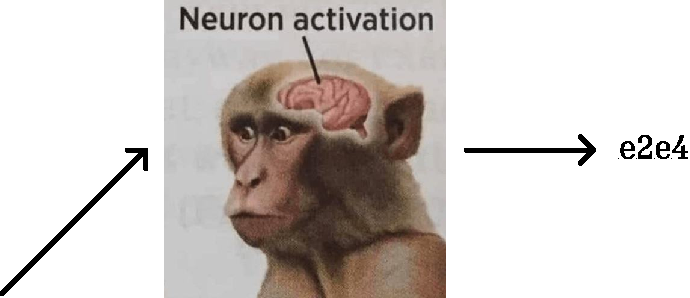
\includegraphics[width=0.8\linewidth]{../assets/slides/human.pdf}}}

            \visible<3->{\subfloat{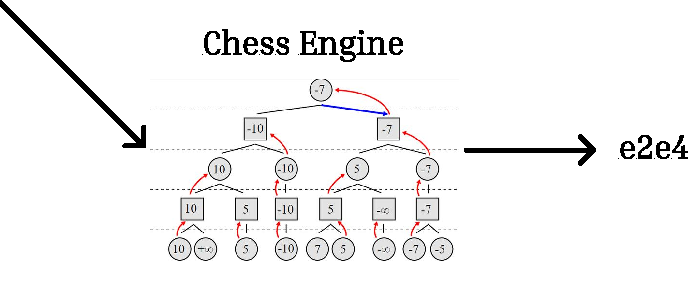
\includegraphics[width=0.8\linewidth]{../assets/slides/computer.pdf}}}
        \end{figure}
    \end{column}
\end{columns}
\end{frame}

\begin{frame}
\frametitle{Ajedrez como árbol}
\begin{figure}
    \centering
    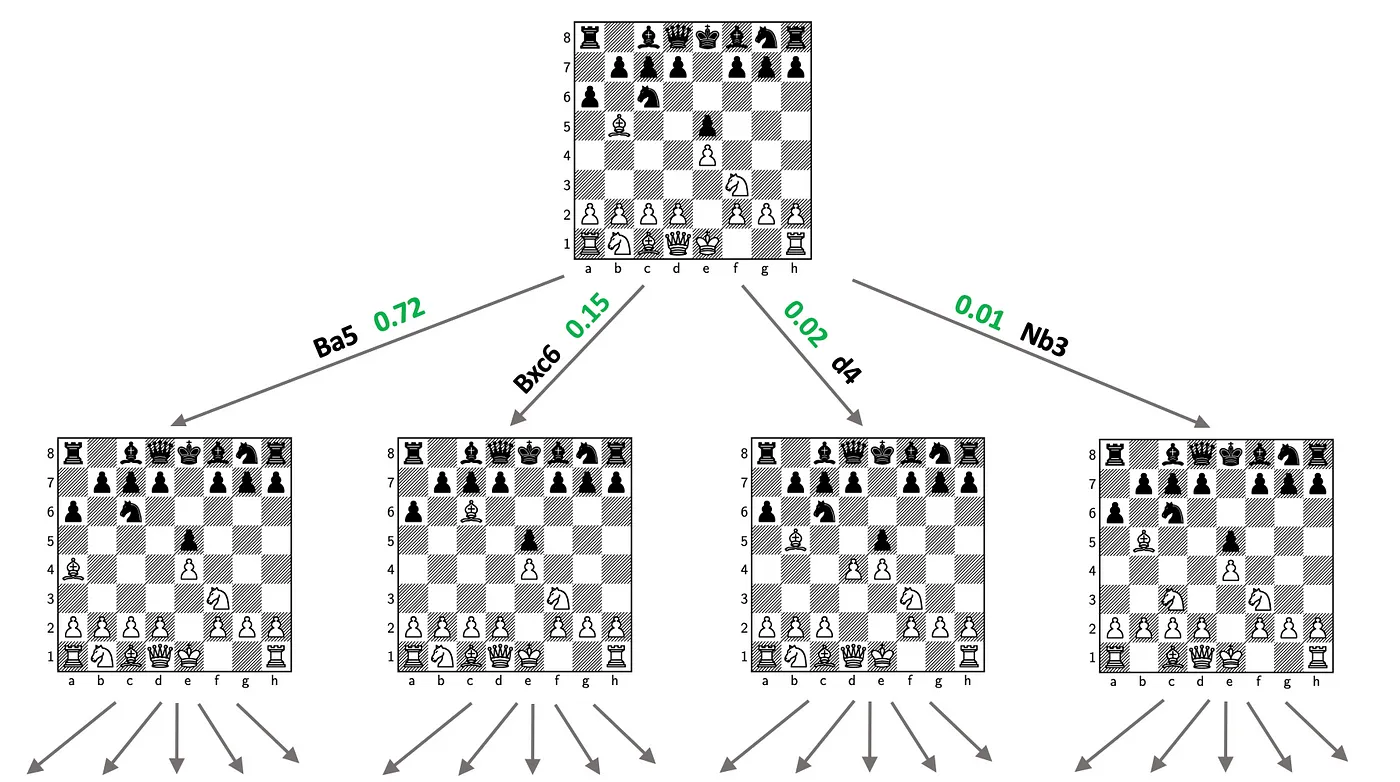
\includegraphics[width=1.0\linewidth]{../assets/slides/chess_tree.png}
\end{figure}
\end{frame}

\begin{frame}
\frametitle{Motores de ajedrez (Chess Engines)}
\begin{columns}
    \begin{column}{0.5\textwidth}
        \begin{itemize}
            \item<1-> Exploran el árbol de juego (Minimax, MCTS, etc.)
            \item<2-> Utilizan funciones de evaluación en las hojas
            \item<3-> La evaluación se propaga hacia arriba, según el algoritmo
        \end{itemize}
    \end{column}
    \begin{column}{0.6\textwidth}
        \begin{figure}
            \centering
            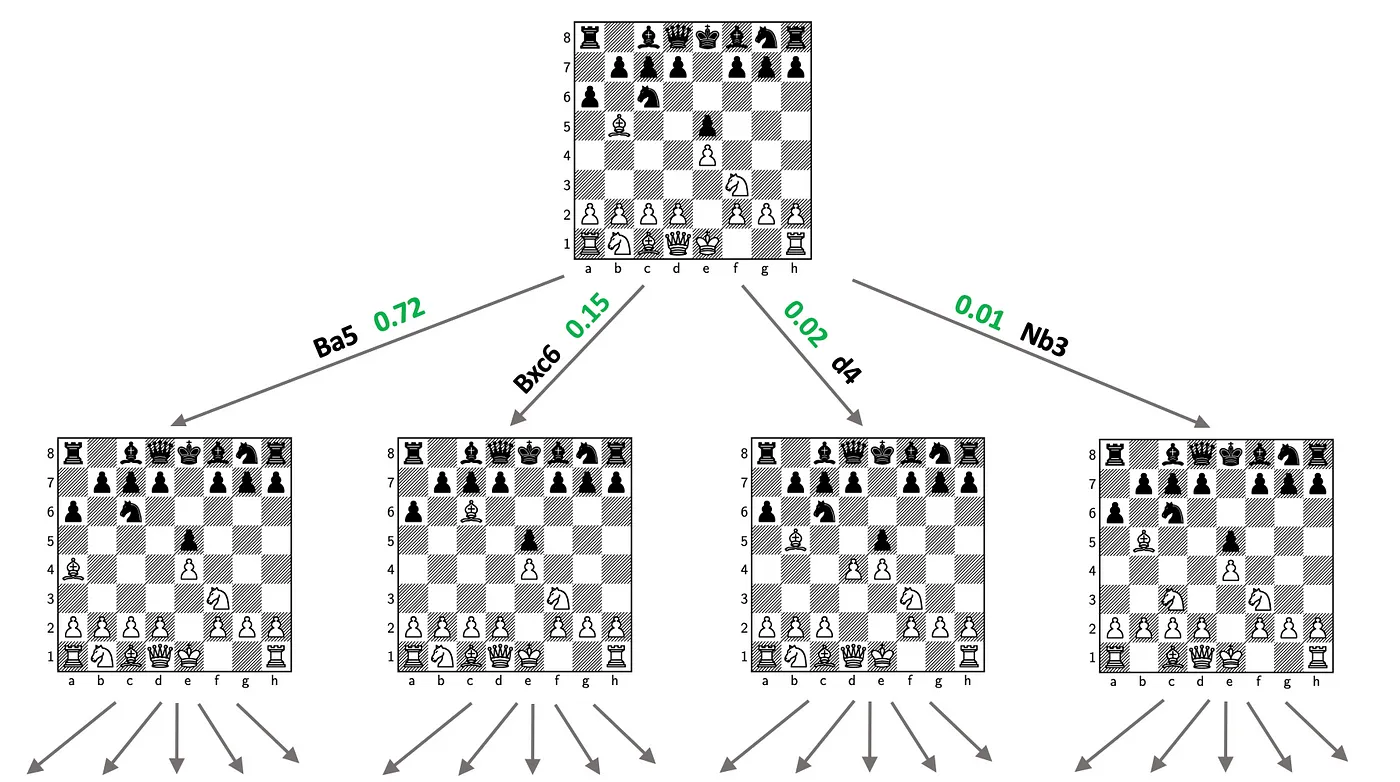
\includegraphics[width=0.9\linewidth]{../assets/slides/chess_tree.png}
        \end{figure}
    \end{column}
\end{columns}
\end{frame}

\begin{frame}
\frametitle{Función de evaluación}
\begin{figure}
    \centering
    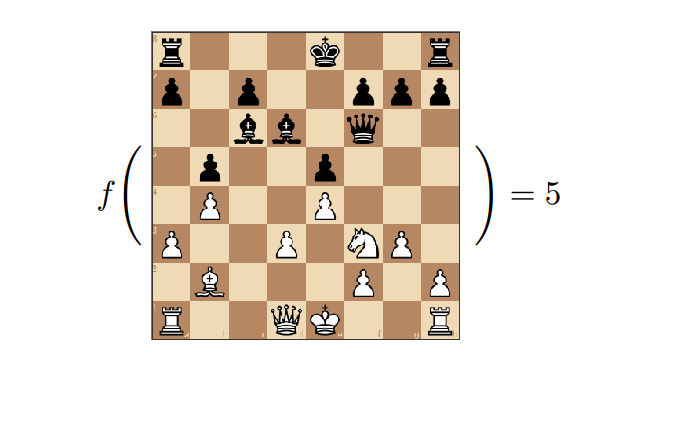
\includegraphics[width=0.8\linewidth]{../assets/slides/eval.png}
\end{figure}
\end{frame}

\begin{frame}
\frametitle{(adelanto) Feature set: ¿Cómo transformar la posición a un vector?}
\begin{figure}
\centering
\includegraphics<1>[width=1.0\linewidth]{../assets/slides/fs_motiv.pdf}
\includegraphics<2>[width=1.0\linewidth]{../assets/slides/fs_motiv2.pdf}
\end{figure}
\end{frame}

\begin{frame}
\frametitle{Motores de ajedrez (breve historia)}


\end{frame}






\begin{frame}
\frametitle{Plan}

asdasd

\begin{itemize}
\item<1-> Text visible on slide 1
\item<2-> Text visible on slide 2
\item<3> Text visible on slide 3
\item<4-> Text visible on slide 4
\end{itemize}

asdasd

\end{frame}


\begin{frame}{Contenido}
\tableofcontents
\end{frame}
